% Created by tikzDevice version 0.12.6 on 2026-05-17 11:03:57
% !TEX encoding = UTF-8 Unicode
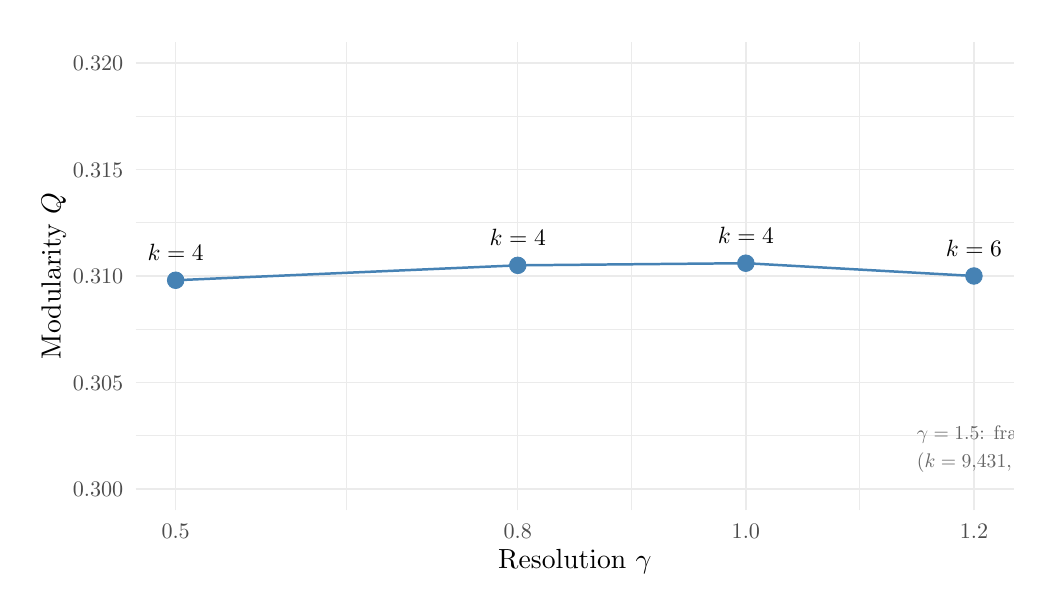
\begin{tikzpicture}[x=1pt,y=1pt]
\definecolor{fillColor}{RGB}{255,255,255}
\path[use as bounding box,fill=fillColor,fill opacity=0.00] (0,0) rectangle (361.35,202.36);
\begin{scope}
\path[clip] (  0.00,  0.00) rectangle (361.35,202.36);
\definecolor{fillColor}{RGB}{255,255,255}

\path[fill=fillColor] ( -0.00,  0.00) rectangle (361.35,202.36);
\end{scope}
\begin{scope}
\path[clip] ( 39.05, 27.90) rectangle (356.35,197.36);
\definecolor{drawColor}{gray}{0.92}

\path[draw=drawColor,line width= 0.3pt,line join=round] ( 39.05, 54.86) --
	(356.35, 54.86);

\path[draw=drawColor,line width= 0.3pt,line join=round] ( 39.05, 93.37) --
	(356.35, 93.37);

\path[draw=drawColor,line width= 0.3pt,line join=round] ( 39.05,131.88) --
	(356.35,131.88);

\path[draw=drawColor,line width= 0.3pt,line join=round] ( 39.05,170.40) --
	(356.35,170.40);

\path[draw=drawColor,line width= 0.3pt,line join=round] (115.28, 27.90) --
	(115.28,197.36);

\path[draw=drawColor,line width= 0.3pt,line join=round] (218.30, 27.90) --
	(218.30,197.36);

\path[draw=drawColor,line width= 0.3pt,line join=round] (300.72, 27.90) --
	(300.72,197.36);

\path[draw=drawColor,line width= 0.5pt,line join=round] ( 39.05, 35.60) --
	(356.35, 35.60);

\path[draw=drawColor,line width= 0.5pt,line join=round] ( 39.05, 74.11) --
	(356.35, 74.11);

\path[draw=drawColor,line width= 0.5pt,line join=round] ( 39.05,112.63) --
	(356.35,112.63);

\path[draw=drawColor,line width= 0.5pt,line join=round] ( 39.05,151.14) --
	(356.35,151.14);

\path[draw=drawColor,line width= 0.5pt,line join=round] ( 39.05,189.65) --
	(356.35,189.65);

\path[draw=drawColor,line width= 0.5pt,line join=round] ( 53.47, 27.90) --
	( 53.47,197.36);

\path[draw=drawColor,line width= 0.5pt,line join=round] (177.10, 27.90) --
	(177.10,197.36);

\path[draw=drawColor,line width= 0.5pt,line join=round] (259.51, 27.90) --
	(259.51,197.36);

\path[draw=drawColor,line width= 0.5pt,line join=round] (341.93, 27.90) --
	(341.93,197.36);
\definecolor{drawColor}{RGB}{70,130,180}

\path[draw=drawColor,line width= 0.9pt,line join=round] ( 53.47,111.09) --
	(177.10,116.48) --
	(259.51,117.25) --
	(341.93,112.63);
\definecolor{fillColor}{RGB}{70,130,180}

\path[draw=drawColor,line width= 0.3pt,line join=round,line cap=round,fill=fillColor] ( 53.47,111.09) circle (  3.00);

\path[draw=drawColor,line width= 0.3pt,line join=round,line cap=round,fill=fillColor] (177.10,116.48) circle (  3.00);

\path[draw=drawColor,line width= 0.3pt,line join=round,line cap=round,fill=fillColor] (259.51,117.25) circle (  3.00);

\path[draw=drawColor,line width= 0.3pt,line join=round,line cap=round,fill=fillColor] (341.93,112.63) circle (  3.00);
\definecolor{drawColor}{RGB}{0,0,0}

\node[text=drawColor,anchor=base,inner sep=0pt, outer sep=0pt, scale=  0.85] at ( 53.47,118.14) {$k=4$};

\node[text=drawColor,anchor=base,inner sep=0pt, outer sep=0pt, scale=  0.85] at (177.10,123.53) {$k=4$};

\node[text=drawColor,anchor=base,inner sep=0pt, outer sep=0pt, scale=  0.85] at (259.51,124.30) {$k=4$};

\node[text=drawColor,anchor=base,inner sep=0pt, outer sep=0pt, scale=  0.85] at (341.93,119.68) {$k=6$};
\definecolor{drawColor}{gray}{0.40}

\node[text=drawColor,anchor=base west,inner sep=0pt, outer sep=0pt, scale=  0.71] at (321.32, 53.68) {$\gamma=1.5$: fragmentation};

\node[text=drawColor,anchor=base west,inner sep=0pt, outer sep=0pt, scale=  0.71] at (321.32, 43.43) {($k=9{,}431$, $Q=0.16$)};
\end{scope}
\begin{scope}
\path[clip] (  0.00,  0.00) rectangle (361.35,202.36);
\definecolor{drawColor}{gray}{0.30}

\node[text=drawColor,anchor=base east,inner sep=0pt, outer sep=0pt, scale=  0.80] at ( 34.55, 32.84) {0.300};

\node[text=drawColor,anchor=base east,inner sep=0pt, outer sep=0pt, scale=  0.80] at ( 34.55, 71.36) {0.305};

\node[text=drawColor,anchor=base east,inner sep=0pt, outer sep=0pt, scale=  0.80] at ( 34.55,109.87) {0.310};

\node[text=drawColor,anchor=base east,inner sep=0pt, outer sep=0pt, scale=  0.80] at ( 34.55,148.38) {0.315};

\node[text=drawColor,anchor=base east,inner sep=0pt, outer sep=0pt, scale=  0.80] at ( 34.55,186.90) {0.320};
\end{scope}
\begin{scope}
\path[clip] (  0.00,  0.00) rectangle (361.35,202.36);
\definecolor{drawColor}{gray}{0.30}

\node[text=drawColor,anchor=base,inner sep=0pt, outer sep=0pt, scale=  0.80] at ( 53.47, 17.89) {0.5};

\node[text=drawColor,anchor=base,inner sep=0pt, outer sep=0pt, scale=  0.80] at (177.10, 17.89) {0.8};

\node[text=drawColor,anchor=base,inner sep=0pt, outer sep=0pt, scale=  0.80] at (259.51, 17.89) {1.0};

\node[text=drawColor,anchor=base,inner sep=0pt, outer sep=0pt, scale=  0.80] at (341.93, 17.89) {1.2};
\end{scope}
\begin{scope}
\path[clip] (  0.00,  0.00) rectangle (361.35,202.36);
\definecolor{drawColor}{RGB}{0,0,0}

\node[text=drawColor,anchor=base,inner sep=0pt, outer sep=0pt, scale=  1.00] at (197.70,  6.94) {Resolution $\gamma$};
\end{scope}
\begin{scope}
\path[clip] (  0.00,  0.00) rectangle (361.35,202.36);
\definecolor{drawColor}{RGB}{0,0,0}

\node[text=drawColor,rotate= 90.00,anchor=base,inner sep=0pt, outer sep=0pt, scale=  1.00] at ( 11.89,112.63) {Modularity $Q$};
\end{scope}
\end{tikzpicture}
